\chapter{System Design}

\section{System Architecture}

This burnout detection system is built using an architecture which comprises several layers including those for collecting data, processing data, performing machine learning tasks, and decision-making.

The system is divided into the following layers: 

\subsection{Data Collection Layer}

This layer is tasked with collecting multi-sourced behavioral data on students. Data is gathered from multiple sources, including academic performance, attendance records, learning management system data, health measures, and social interaction networks.

The data collected is then saved in one main database for further analysis. The issue of data confidentiality is observed by adopting various data anonymization methods.

\subsection{Data Processing Layer}

At this stage, the raw data undergo preprocessing, where missing values are addressed, inconsistencies are resolved, and numerical attributes are scaled. 
Feature extraction and transformation is employed to transform raw behavioral data into structured data that can be used by machine learning algorithms.

\subsection{Feature Engineering Layer}

Provides feature extraction of elements that are important in relation to the processed data. Patterns in the temporal behavior and data are established to create important features, including engagement, stress, and academic performance trends.

It is also possible to create composite features for behavioral patterns like academic stress and social withdrawal.

\subsection{Machine Learning Layer}

The machine learning component is made up of several prediction models that have been trained to identify early symptoms of burnout. Various algorithms like Logistic Regression, Random Forest, Gradient Boosting, and Support Vector Machines are deployed for comparison purposes.

These models are trained using past behavioral information and validated through cross-validation.

\subsection{Prediction and Decision Layer}

This layer calculates the burnout probability score and categorizes the users based on their risk of burnout. Depending on the risk level identified, the system makes valuable suggestions.

The decision layer allows for the early identification of potential burnout cases to prevent an impending crisis.

\subsection{Visualization and Interface Layer}

The last layer displays results in dashboards or reporting systems. Administrators and counselors can view the risks, trends, and alerts in this layer.
This layer enhances user-friendliness and supports evidence-based decision-making.

\textbf{[Insert System Architecture Diagram Here]}


\section{System Workflow}

The process workflow refers to the steps that have to be followed during the burnout identification process. The process begins by collecting raw behavior data from different sources.

Once the data has been collected, it is subjected to pre-processing. During this phase, the inconsistencies in the data are sorted out, and normalization is conducted.

The features obtained from the pre-processed data are further analyzed through feature engineering. This step ensures that the necessary features are extracted. Such features include engagement score, stress levels, and academic trends.

The features obtained from feature engineering are fed into machine learning algorithms to obtain the probability of experiencing burnout.

Finally, the outputs obtained from the process are used to identify different user groups. Each group is assigned actions, which include displaying the results on a visualization screen.

\textbf{[Insert Workflow Diagram Here]}


\section{Data Flow Diagram}





\section{Use Case Diagram}

\begin{figure}
    \centering
    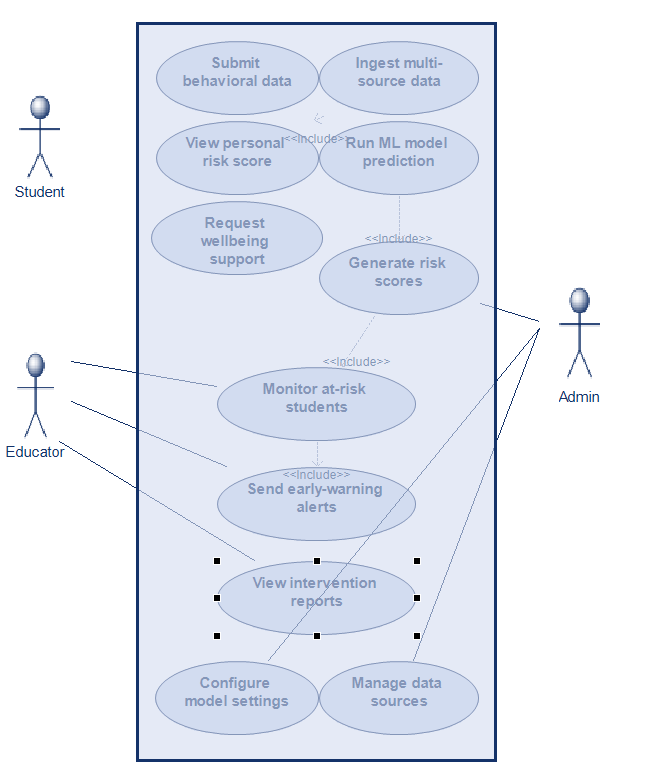
\includegraphics[width=0.7\linewidth]{image.png}
    \caption{use case diagram of burnout signal detection}
    \label{fig:placeholder}
\end{figure}

\section{Class Diagram}




\section{Sequence Diagram}



\textbf{[Insert Sequence Diagram Here]}


\section{Design Considerations}

The system will incorporate the following characteristics:

\begin{itemize}
    \item \textbf{Scalability:} The ability to manage large amounts of data about students and work under institutional settings
    \item \textbf{Accuracy:} High accuracy of predictions through sophisticated machine learning algorithms
    \item \textbf{Security:} The ability to process data securely
    \item \textbf{Modularity:} Distinctiveness between different system components
    \item \textbf{Real-time Processing:} Enables constant monitoring and prediction
\end{itemize}